\chapter{Other Cloud Mechanisms}
Le risorse IT cloud-based necessitano di essere configurate, impostate, e soprattutto sono soggette molto spesso a manutenzione. In questo capitolo sono illustrati alcuni meccanismi che riguardano questo tipo di attività, e che riguardano la sicurezza, e in particolare distingueremo i meccanismi in \textit{Cloud Management Mechanisms} e \textit{Cloud Security Mechanisms}.

\section{Cloud Management Mechanisms}
Dei primi fanno parte: Remote Administration System, Resource Management System, SLA Management System, Billing Management System.

\subsection{Remote Administration System}
È un meccanismo che fornisce strumenti e interfacce utente per i cloud resource administrator esterni per configurare e amministrare le risorse IT cloud-based. Gli strumenti e le API messe a disposizione da un remote administration system sono utilizzate dal cloud provider per sviluppare e personalizzare i portali online che forniscono poi al cloud consumer con una varietà di controlli di amministrazione. I due tipi principali di portali sono:
\begin{itemize}
    \item \textbf{Usage and Administration Portal} - un portale general purpose che permette ai cloud consumer di centralizzare la gestione dei controlli di diverse risorse IT cloud-based.
    \item \textbf{Self-Service Portal} - è una specie di portale shopping che permette ai cloud consumer di cercare in una lista di servizi cloud e risorse IT messe a disposizione dal cloud provider quello che più si avvicina ai loro requisiti.
\end{itemize}

\begin{figure}[ht]
    \centering
    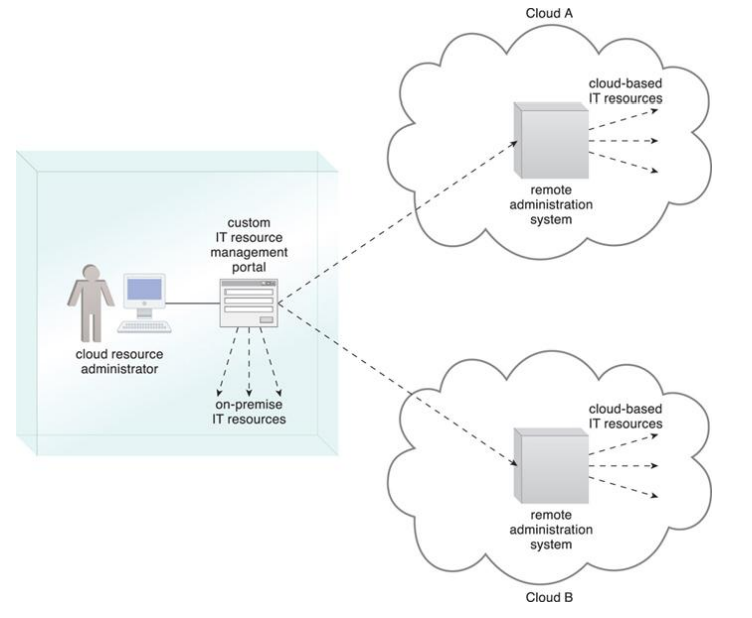
\includegraphics[width=9cm]{./Images/cap10/10.1.png}
\end{figure}

\subsection{Resource Management System}
È un meccanismo che aiuta a coordinare l'utilizzo delle risorse IT a seguito di azioni di gestione fatte dai consumer e dai provider. Tutto ciò è possibile grazie alla VIM che coordina l'hardware dei server, ad esempio creando istanze multiple di un hypervisor a cavallo di diversi server fisici. Le attività che normalmente sono automatizzate tramite il Resource Management System sono:
\begin{itemize}
    \item gestione dei template delle risorse IT virtuali che sono utilizzate per creare istanze preconfigurate;
    \item allocazione e rilascio di risorse IT virtuali nelle infrastrutture fisiche in risposta alla terminazione o la messa in pausa di altre risorse IT virtuali;
    \item coordinazione delle risorse IT in relazione al coinvolgimento di nuovi meccanismi come resource replication, load balancer e failover system.
\end{itemize}
Le funzioni di gestione possono essere accessibili sia dal cloud consumer che dai cloud provider, e tipicamente espongono delle API che permettono ai cloud provider di costruire sistemi di amministrazione remota che possono essere personalizzati per gestire meglio il controllo delle risorse.

\subsection{SLA Management System}
Rappresenta una serie di prodotti commerciali disponibili che forniscono funzioni riguardanti l'amministrazione, la collezione, lo storage, il reporting e la notifica dei dati degli SLA. Il deployment di un SLA management system di solito include una repository usata per salvare e per recuperare i dati di un SLA basati su metriche predefinite e parametri di reporting.

\begin{figure}[htb!]
    \centering
    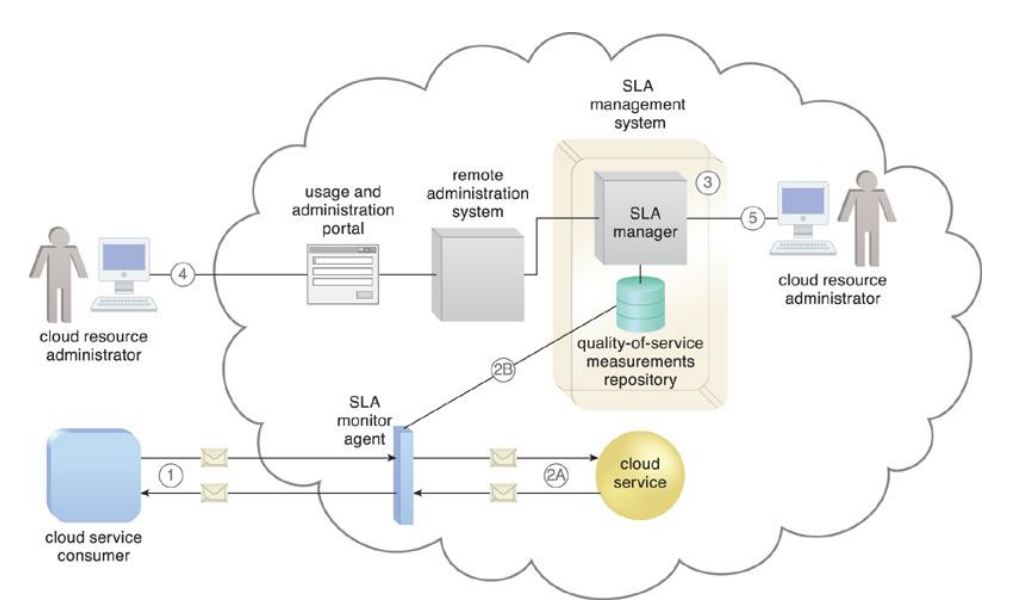
\includegraphics[width=9cm]{./Images/cap10/10.2.png}
\end{figure}
\clearpage

\subsection{Billing Management System}
È un meccanismo dedicato alla collezione e al processing dei dati di utilizzo che riguardano la gestione degli account da parte del cloud provider e la fatturazione da parte del cloud consumer. Nello specifico, il billing management system si basa su dei monitor pay-per-use per acquisire dati di utilizzo durante l'esecuzione che sono salvati in repository che le componenti del sistema raccolgono per propositi di fatturazione. Grazie a questo meccanismo è possibile personalizzare l'utilizzo di certe risorse e stabilire dei modelli di prezzo personalizzati.


\section{Cloud Security Mechanisms}
I meccanismi di sicurezza affrontati in questa sezione tornano utili per affrontare le minacce affrontate nei capitoli precedenti e per migliorare l'affidabilità di un ambiente cloud. 

\subsection{Encryption}
I dati normalmente sono codificati in un formato leggibile chiamato \textit{plaintext} (testo in chiaro). Il testo in chiaro è vulnerabile ad attacchi quando trasmesso su canali insicuri, per cui si utilizza il meccanismo della crittografia (encryption): serve a preservare la confidenzialità e l'integrità dei dati. Questo meccanismo si basa su un algoritmo di cifratura che trasforma il testo in chiaro in un cifrato (ciphertext). Quando viene applicato un algoritmo di cifratura, si utilizza una stringa di caratteri chiamata \textbf{chiave di cifratura}, che è stabilita precedentemente e scambiata tra le parti interessate. La chiave viene poi utilizzata per decifrare il cifrato nel testo in chiaro. Ci sono due tipi di cifratura: simmetrica e asimmetrica.

\subsubsection{SYMMETRIC ENCRYPTION}
La cifratura simmetrica usa la stessa chiave per cifrare e per decifrare: queste due funzioni sono eseguite da entrambi i partecipanti alla discussione. Viene eseguito sempre un controllo di autenticazione perché solo le parti autorizzate che posseggono la chiave possono generare i messaggi. Questo tipo di cifratura non ha la caratteristica nel non ripudio, perché se qualcun altro entra in possesso della chiave può inviare anch'esso messaggi.

\subsubsection{ASYMMETRIC ENCRYPTION}
La cifratura asimmetrica, chiamata anche crittografia a chiave pubblica, si basa sull'utilizzo di due chiavi, ovvero chiave pubblica e chiave privata. La prima è di dominio pubblico mentre la seconda è nota solo al proprietario: per cifrare un messaggio si utilizza la chiave pubblica di Bob, e quel messaggio può essere decifrato solo con la chiave privata di Bob. Il fatto che ci siano due chiavi anziché una fa sì che la crittografia asimmetrica sia più lenta computazionalmente di quella a chiave privata.

\begin{mdframed}[backgroundcolor=gray!20,shadow=false]
Il meccanismo di crittografia, quando usato per mettere al sicuro le trasmissioni web, è applicato di norma tramite via HTTPS, il quale fa uso di SSL e TLS tramite HTTP. Il protocollo TLS (\textit{transport layer security}) è il successore del SSL (\textit{secure socket layer}). Dato che la crittografia asimmetrica è più time-consuming di quella simmetrica, il protocollo TLS usa il primo solo per lo scambio di chiavi, e poi passa alla modalità simmetrica.
\end{mdframed}

\subsection{Hashing}
È usato quando viene richiesto un tipo di protezione univoca, senza possibilità di tornare indietro. Una volta che l'hash viene applicato ad un messaggio, viene bloccato e non viene fornita alcuna chiave. Un caso d'uso di questa tecnologia è nello storage delle password. Per controllare se un messaggio è integro, si calcola l'hash e si confronta con quello ricevuto.

\subsection{Digital Signature}
La firma digitale serve a fornire autenticità e integrità attraverso autenticazione e non ripudio. A un messaggio viene assegnata una firma digitale prima della sua trasmissione, la quale viene resa non valida nel caso di modifiche non autorizzate al messaggio. La firma digitale rappresenta una prova che il messaggio ricevuto è lo stesso che è stato inviato dal mittente. Nella costruzione di una firma digitale vengono utilizzati sia l'hashing che la crittografia asimmetrica, e questo meccanismo viene utilizzato per evitare le minacce di \textit{malicious intermediary}, \textit{insufficient authorization} e \textit{overlapping trust boundaries}.

\begin{figure}[htb!]
    \centering
    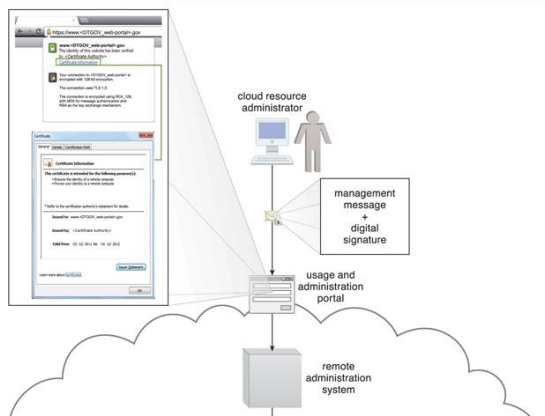
\includegraphics[width=8cm]{./Images/cap10/10.3.png}
\end{figure}


\subsection{Public Key Infrastructure (PKI)}
Rappresenta un approccio comune per gestire le problematiche delle chiavi asimmetriche: consiste in una serie di protocolli e regole che permettono a sistemi molto grandi di utilizzare in modo sicuro la crittografia a chiave pubblica. Il PKI si basa sui certificati digitali, che sono strutture dati firmate digitalmente che uniscono tra loro le chiavi pubbliche per certificare l'identità del loro possessore. I certificati digitali spesso sono firmati da una terza parte rappresentata da una CA (\textit{Certificate Authority}), come mostrato nella figura alla pagina successiva.

\begin{figure}[htb!]
    \centering
    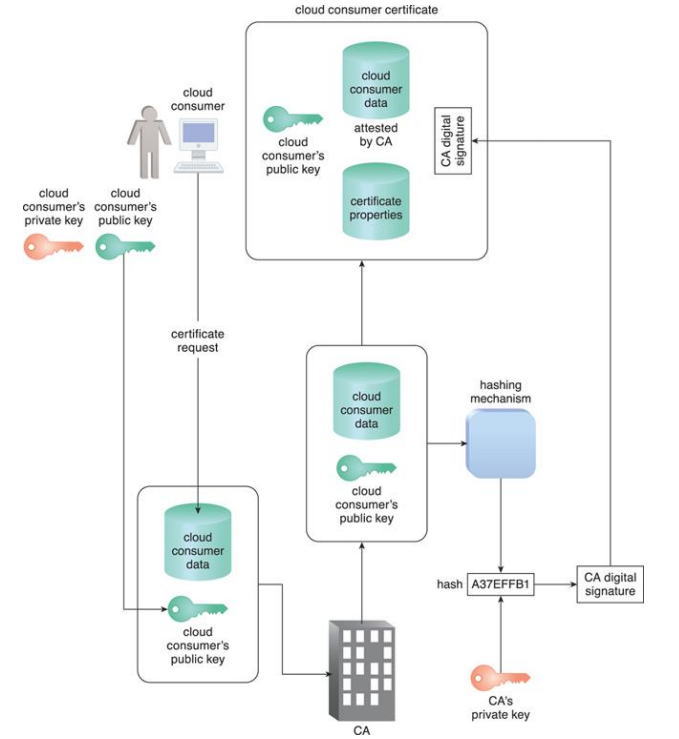
\includegraphics[width=9cm]{./Images/cap10/10.4.png}
\end{figure}

\vspace{5mm}

Alcune CA molto famose sono VeriSign e Comodo, ma capita anche che grandi aziende come Microsoft pubblichino i loro certificati. Un certificato può essere tuttavia generato da chiunque, a patto che abbia a disposizione gli strumenti giusti. Il PKI viene usato per contrastare la minaccia di \textit{insufficient authorization}.

\subsection{Identity and Access Management (IAM)}
Utilizza le componenti e le policy necessarie per controllare e tracciare gli utenti, le loro identità e i loro privilegi di accesso per le risorse, gli ambienti e i sistemi. In particolare, il meccanismo di IAM comprende quattro componenti principali:
\begin{itemize}
    \item \textbf{Authentication} - le combinazioni username/password restano la forma più comune di credenziali di accesso gestite dall'IAM, che supporta anche firme digitali o metodi di autenticazione biometrica, come le impronte digitali.
    \item \textbf{Authorization} - definisce la giusta granularità per il controllo degli accessi e riguarda anche la relazione tra le identità e i privilegi di accesso a una risorsa IT o ad una componente.
    \item \textbf{User Management} - riguarda le capacità di amministratore del sistema, che può creare profili, assegnare ruoli, modificare privilegi.
    \item \textbf{Credential Management} - la gestione delle credenziali stabilisce le identità e i ruoli per gli account già esistenti.
\end{itemize}
IAM viene usato per contrastare le minacce di \textit{insufficient authorization}, \textit{denial of service} e \textit{overlapping trust boundaries}.

\subsection{Single Sign-On (SSO)}
La propagazione delle autenticazioni e delle informazioni sulle autorizzazioni per un cloud service consumer attraverso diversi servizi cloud può essere problematico, soprattutto se diverse risorse e servizi devono essere invocati per una stessa routine. Il meccanismo di Single Sign-On permette ad un cloud service consumer di essere autenticato da un security broker, che stabilisce un contesto di sicurezza che persiste durante l'utilizzo di servizi che si trovano in punti diversi del cloud. Nonostante non migliora la sicurezza del sistema, e non combatte nessuna minaccia,  migliora di molto l'usabilità in quanto evita al consumer di autenticarsi ogni volta.

\subsection{Cloud-Based Security Groups}
Come può sembrare scontato, alzare delle barriere tra i dati aumenta la protezione degli stessi. La segmentazione delle risorse cloud-based è un processo che separa gli ambienti fisici da quelli virtuali che sono creati per diversi utenti o gruppi, come abbiamo visto già molte volte. Vengono definite delle policy per ogni gruppo basate sulle condizioni di utilizzo o sugli obiettivi comuni, e vengono dati dei permessi per utilizzare determinate risorse piuttosto che altre. Ad esempio diversi server virtuali che girano su uno stesso server fisico possono essere membri di due security group diversi. Il cloud resource administrator è colui che si occupa di questa divisione.

\begin{figure}[htb!]
    \centering
    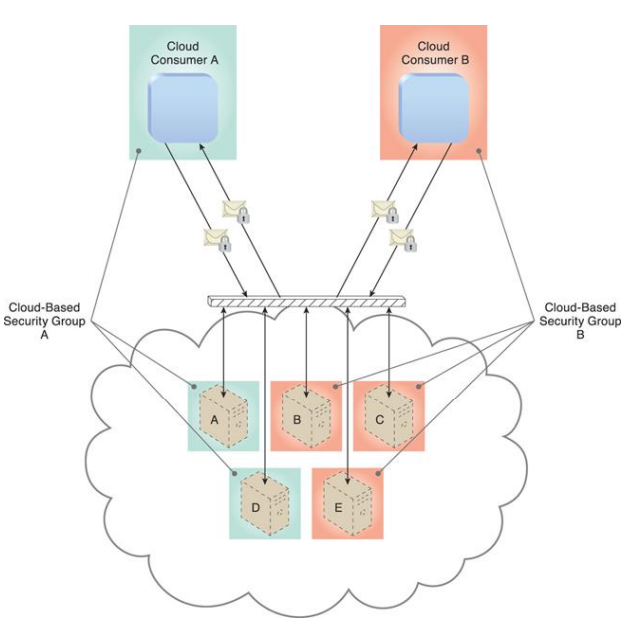
\includegraphics[width=8cm]{./Images/cap10/10.5.png}
\end{figure}

Questo meccanismo può essere utilizzato per combattere le minacce di \textit{denial of service} e \textit{overlapping trust boundaries}, ed è molto simile al concetto di \textbf{Logical Network Perimeter}.


\subsection{Hardened Virtual Server Images}
Come abbiamo visto in precedenza, le macchine virtuali in un ambiente cloud, tra cui anche i server, vengono generate a partire da un file immagine preconfigurato, in modo da migliorare prestazioni e usabilità. Le \textit{Hardened Virtual Server Images} sono dei template per la creazione di macchine virtuali a cui è stata migliorata la robustezza disabilitando ad esempio porte inutilizzate, servizi inutili o software ridondanti. Questo meccanismo combatte le minacce di \textit{denial of service}, \textit{insufficient authorization} e \textit{overlapping trust boundaries}.


\section{Learning Check}
\begin{enumerate}
    \item Descrivi il meccanismo di Remote Administration System e spiega la sua relazione con i sistemi di fatturazione e con i SLA.
    \item Descrivi gli obiettivi del meccanismo di Resource Management System ed elenca i task comuni che possono essere portati a termine con esso.
    \item Descrivi gli obiettivi del meccanismo di SLA Management System e spiega come è in relazione con il meccanismo di SLA Monitor. Inoltre illustra l'importanza dell'elaborazione dell'utilizzo dei dati in relazione alle garanzie presenti in un SLA.
    \item Descrivi gli obiettivi del meccanismo di Billing Management System e spiega la sua relazione con il meccanismo di Pay-Per-Use Monitor.
    \item Descrivi il meccanismo di Encryption Security e spiega come funziona in relazione a testo in chiaro, testo cifrato e chiavi condivise. Inoltre spiega come le cifrature possono essere applicate si all'interno che all'esterno dei cloud boundaries.
    \item Elenca le possibili minacce alla sicurezza che possono verificarsi in seguito alla cifratura.
    \item Descrivi il meccanismo di Hashing e spiega la sua relazione con i meccanismi di cifratura.
    \item Elenca le possibili minacce alla sicurezza che possono verificarsi in seguito all'hashing.
    \item Descrivi il meccanismo Digital Signatures Security e spiega come funzionano le firme digitali in relazione ad autenticazione e integrità. Inoltre spiega come le firme digitali possono essere applicate si all'interno che all'esterno dei cloud boundaries.
    \item Elenca le possibili minacce alla sicurezza che possono verificarsi in seguito all'utilizzo di firme digitali.
    \item Descrivi il meccanismo di Public Key Infrastructure (PKI) e la sua relazione con i meccanismi appena illustrati.
    \item Elenca le possibili minacce alla sicurezza che possono verificarsi in seguito all'utilizzo di PKI.
    \item Descrivi il meccanismo di IAM (Identity and Access Management) e spiega l'obiettivo del salvataggio dell'identità messo in atto da un IAM. Inoltre spiega come un IAM può stabilire ruoli e regole.
    \item Elenca le possibili minacce alla sicurezza che possono verificarsi in seguito all'utilizzo di IAM.
    \item Descrivi il meccanismo di Single Sign-On e descrivi l'obiettivo del Security Broker. Spiega inoltre perché questo meccanismo non ha a che fare direttamente con le minacce alla sicurezza viste in precedenza.
    \item Descirivi il meccanismo di Cloud-Based Security Groups e come questi gruppi sono messi insieme logicamente e non fisicamente. Inoltre spiega come possono essere assegnate le risorse IT ai gruppi.
    \item Elenca le possibili minacce alla sicurezza che possono verificarsi in seguito all'utilizzo del meccanismo di Cloud-Based Security Groups.
    \item Descrivi il meccanismo di Hardened Virtual Server Images e spiega come l'immagine di un virtual server può essere resa più robusta per questioni di sicurezza.
    \item Elenca le possibili minacce alla sicurezza che possono verificarsi in seguito all'utilizzo del meccanismo di Hardened Virtual Server Images.
\end{enumerate}
